\documentclass{report} 
\title{Strang}
\date{Started 5th June 2025}
\author{Malcolm}
\usepackage{amsmath} %import math
\usepackage{mathtools} %more math
\usepackage{amssymb} %for QED symbol
\usepackage{amsthm} %
\usepackage{bm}%bold math
\usepackage{graphicx} %import imaging
\graphicspath{{./images/}} %set imaging path
\begin{document}
\maketitle

\tableofcontents

\newpage

\chapter{Vectors and Matrices}
\section{Intuition for Dot product, Cosine formula, Schwarz and Triangle inequalities}
\textbf{Intuition for dot product}\\
The unit vectors $\bm{v}=(\cos\alpha,\sin\alpha)$ and $\bm{w}=(\cos\beta,\sin\beta)$ are plotted as follows
\begin{center}
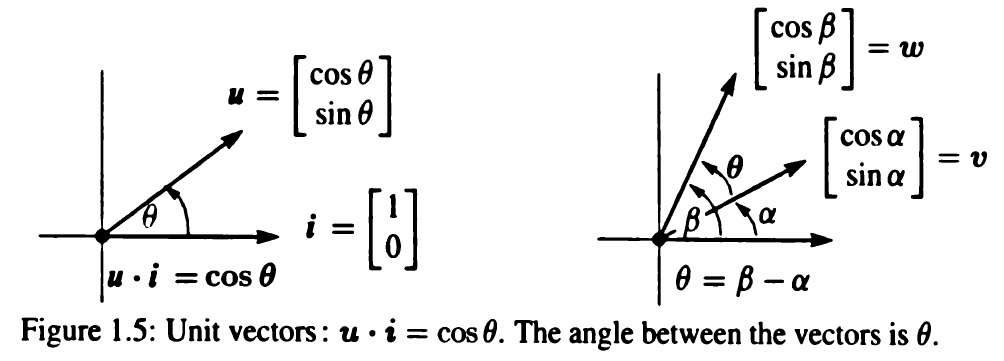
\includegraphics[width=10cm]{1}
\end{center}
See first that when fixed in this form, the magnitude of both vectors is 1, with an angle $\beta-\alpha$ between them. These unit vectors have dot product
\begin{equation*}
\bm{v}\cdot\bm{w}=\cos\alpha\cos\beta+\sin\alpha\sin\beta=\cos(\beta-\alpha)
\end{equation*}
We have $\theta$ as the angle between the two vectors; see that the sign of $\bm v\cdot\bm w$ tells us whether $\theta$ is below or above a right angle (due
to the cosine function being negative for its argument $>\pi/2$ and positive for $<\pi/2$):
\begin{center}
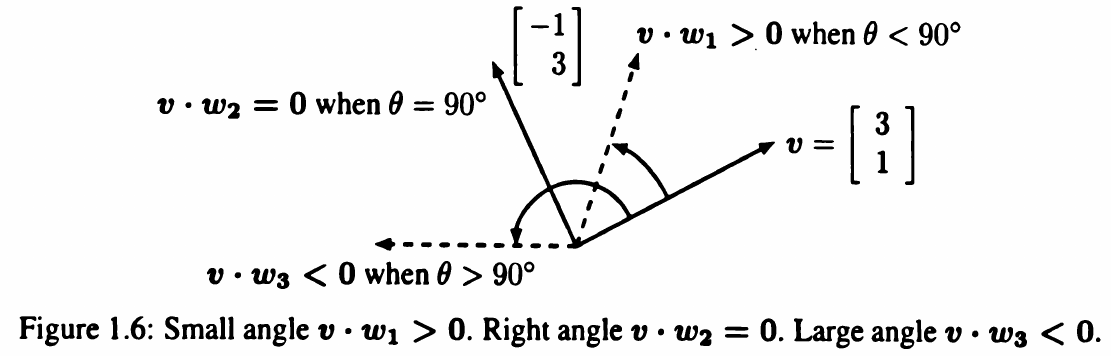
\includegraphics[width=9cm]{2}
\end{center}
(next page)\newpage
\noindent\textbf{Cont.}\\
The idea here is that the dot product reveals the exact angle $\theta$; for unit vectors $\bm u$ and $\bm U$, the dot product $\bm u\cdot\bm U$ is the cosine of 
$\theta$. Ths remains true in $n$ dimensions (not shown).\\
\vspace{1mm}\\
See that any $\bm{u}$ and $\bm{v}$ can be fixed in the above form by normalising their lengths to get
$\bm u=\bm v/||\bm v||$ and $\bm U=\bm w/||\bm w||$. After which their dot product would give $\cos\theta$. This leads us to the \textit{cosine formula}:
\begin{equation*}
\text{\textbf{Cosine formula}: }
\frac{\bm v\cdot\bm w}{||\bm v||\,||\bm w||}=\cos\theta\quad\text{ if $\bm v$ and $\bm w$ are nonzero vectors}
\end{equation*}
\textbf{Perpendicular vectors}\\
See that when the angle between $\bm v$ and $\bm w$ is $90^\circ$, its cosine is 0; this gives us a way to test this. Also see that for perpendicular vectors:
\begin{equation*}
||\bm v+\bm w||^2=||\bm v||^2+||\bm w||^2
\end{equation*}
because
\begin{equation*}
||\bm v+\bm w||^2=(\bm v+\bm w)\cdot(\bm v+\bm w)=\bm v\cdot\bm v+\bm v\cdot\bm w+\bm w\cdot\bm v+\bm w\cdot\bm w
\end{equation*}
where $\bm v\cdot \bm w=0$.\\
\vspace{1mm}\\
\textbf{Schwarz and Triangle inequalities}\\
First, see from the cosine formula that the dot product of $\bm v/||\bm v||$ and
$\bm w/||\bm w||$ never exceeds one (since $\cos\theta$ never exceeds one). This is the the 
\textit{Schwarz inequality}:
\begin{equation*}
\text{\textbf{Schwarz inequality}: }|\bm v\cdot\bm w|\leq||\bm v||\,||\bm w||
\end{equation*}
The \textit{Triangle inequality} comes directly from the Schwarz inequality:
\begin{equation*}
\text{\textbf{Triangle inequality}: }||\bm v+\bm w||\leq||\bm v||+||\bm w||
\end{equation*}
This can be seen from
\begin{equation*}
||\bm v+\bm w||^2=\bm v\cdot\bm v+\bm v\cdot\bm w+\bm w\cdot\bm v+\bm w\cdot\bm w
\leq||\bm v||^2+2||\bm v||\,||\bm w||+||\bm w||^2
\end{equation*}
The square root gives us the triangle equality (side 3 cannot exceed side 1 + side 2).
\newpage

\section{Intuition for column rank being equal to row rank}
If all columns are in the same direction, why does it happen that all the rows are the same direction?\\
\vspace{1mm}\\
Consider the matrix, see that column 2 is $m$ times column 1:
\begin{equation*}
\bm A=\left[\begin{array}{cc}
a&ma\\
b&mb
\end{array}\right]
\end{equation*}
See that the second row is just $b/a$ times the first row---if the column rank is 1, then the row rank is 1. See that transposing the matrix, we have
\begin{equation*}
\bm A=\left[\begin{array}{cc}
a(1)&b(1)\\
a(m)&b(m)
\end{array}\right]
\end{equation*}
which still has one independent column. Now consider the 3x3 case:
\begin{equation*}
\bm A=\left[\begin{array}{ccc}
a&ma&pa\\
b&mb&pb\\
c&mc&pc
\end{array}\right]
\end{equation*}
See that a similar deduction can also be made in this case, where the row rank of $A$ is equal to its column rank.\\
(next page)\newpage
\noindent\textbf{An informal proof}\\
Consider any matrix $\bm A$, suppose we go from left to right, looking for independent columns of $\bm A$ using the following procedure:
\begin{enumerate}
\item If column 1 of $\bm A$ is not zero, put it in matrix $\bm C$
\item If column 2 of $\bm A$ is not a multiple of column 1, put it in into $\bm C$
\item If column 3 of $\bm A$ is not a combination of columns 1 and 2, put it into $C$. \textit{continue}
\end{enumerate}
See that at the end $\bm C$ will have $r$ columns taken from $\bm A$, where $r$ is the rank of $\bm A$ and $\bm C$. While the $n$ columns of $\bm A$ are dependent, 
the $r$ columns of $\bm C$ will surely be independent.\\
\vspace{1mm}\\
For instance consider $\bm A$ with rank 2
\begin{equation*}
\bm A=\left[\begin{array}{ccc}
2&6&4\\
4&12&8\\
1&3&5
\end{array}\right]\quad\text{leads to}\quad \bm C=
\left[\begin{array}{cc}
2&4\\
4&8\\
1&5
\end{array}\right]
\end{equation*}
Now consider another matrix $\bm R$ to be multiplied by $\bm C$ such that 
$\bm A=\bm{CR}$. The first and third columns of $\bm A$ are already in $\bm C$, so those respective columns in $\bm R$ make up a \textit{identity matrix};
the second column of $\bm A$ is a multiple of the first, so we have
\begin{equation*}
\bm A=\bm{CR}\quad\text{is }\left[\begin{array}{ccc}
2&6&4\\
4&12&8\\
1&3&5
\end{array}\right]=
\left[\begin{array}{cc}
2&4\\
4&8\\
1&5
\end{array}\right]
\left[\begin{array}{ccc}
1&3&0\\
0&0&1
\end{array}\right]
\end{equation*}
(See that the $i$th row of $\bm A$ can be seen as a linear combination of the rows of $\bm R$ specified the $i$th row of $\bm C$. 
(or just consider $\bm A^T=\bm R^T\bm C^T$). We know that
\begin{enumerate}
\item $\bm C$ contains the full set of $r$ independent columns of $\bm A$.
\item $\bm R=[\bm{I\,\bm F}]$ contains the identity matrix $\bm I$ in the same $r$ columns that held $\bm C$.
\item The dependent columns of $\bm A$ are combinations of $\bm{CF}$ of the independent columns in $\bm C$.
\end{enumerate}
Where the matrix $\bm F$ goes into the other $n-r$ columns of $\bm R=[\bm{I\,\bm F}]$. ($\bm A=\bm{CR}$ becomes $\bm A=\bm{C[I,F]}=\bm{[C,CF]}=
[\text{indep cols of $\bm A$},\text{ dep cols of $\bm A$}]$ (in correct order).\\
\vspace{1mm}\\
See that $\bm C$ has the same column space as $\bm A$, and $\bm R$ \textit{has the same row space} as $\bm A$ (every row of $\bm A$ is a combination of the rows
of $\bm R$).\\
(next page)\newpage
\noindent\textbf{Cont.}\\
We had the example
\begin{equation*}
\bm A=\bm{CR}\quad\text{is }\left[\begin{array}{ccc}
2&6&4\\
4&12&8\\
1&3&5
\end{array}\right]=
\left[\begin{array}{cc}
2&4\\
4&8\\
1&5
\end{array}\right]
\left[\begin{array}{ccc}
1&3&0\\
0&0&1
\end{array}\right]
\end{equation*}
\textit{Here is an informal proof that the row rank of $\bm A$ equals the column rank of $\bm A$} (based from facts we already know)
\begin{enumerate}
\item The $r$ columns of $\bm C$ are independent (chosen that way from $\bm A$)
\item Every column of $\bm A$ is a combination of those $r$ columns of $\bm C$ (since $\bm A=\bm{CR}$)
\item The $r$ rows of $\bm R$ are independent (they contain the $r$ by $r$ matrix $\bm I$)
\item Every row of $\bm A$ is a combination of the $\bm r$ rows of $\bm R$
\end{enumerate}
See that for every column of $\bm A$ that goes into $\bm C$, a column of $\bm I$ goes into $\bm R$, where each column of $\bm I$ in $\bm R$ adds an independent row.\\
\vspace{1mm}\\
This means that the column rank of $\bm C$ (column space of $\bm A$) is always equal to the row rank of $\bm R$ (row space of $\bm A$)---the 
column rank of $\bm A$ is equal to the row rank of $\bm A$.\\
\vspace{1mm}\\
\textbf{More examples}\\
Rank 2:
\begin{equation*}
\left[\begin{array}{ccc}
1&2&3\\
4&5&6\\
7&8&9
\end{array}\right]=
\left[\begin{array}{cc}
1&2\\
4&5\\
7&8
\end{array}\right]
\left[\begin{array}{ccc}
1&0&-1\\
0&1&2
\end{array}\right]
\end{equation*}
Rank 2:
\begin{equation*}
\left[\begin{array}{cccc}
1&2&3&4\\
1&2&4&5
\end{array}\right]=
\left[\begin{array}{cc}
1&3\\
1&4
\end{array}\right]
\left[\begin{array}{cccc}
1&2&0&1\\
0&0&1&1
\end{array}\right]
\end{equation*}
Rank 1:
\begin{equation*}
\left[\begin{array}{cccc}
1&2&10&100\\
3&6&30&300\\
2&4&20&200
\end{array}\right]=
\left[\begin{array}{c}
1\\3\\2
\end{array}\right]
\left[\begin{array}{cccc}
1&2&10&100
\end{array}\right]
\end{equation*}
\newpage

\section{Ways to multiply $\bm{AB}=\bm C$}
\textbf{Multiplcation by columns of $\bm A$ and rows of $\bm B$}\\
A lesser known way to multiply $\bm{AB}$ is through considering the columns of $\bm A$ and the rows of $\bm B$ (contrary to the usual ideas where each 
entry of the result is a dot product of a row of $\bm A$ and column of $\bm B$):
\begin{center}
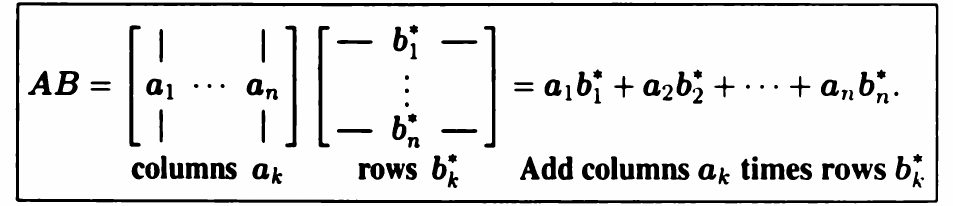
\includegraphics[width=10cm]{3}
\end{center}
We multiply each column of $\bm A$ by each row of $\bm B$; this gives us $n$ rank 1 matrices, which we then sum together; these matrices are called \textit{outer products}\\
\vspace{1mm}\\
(usually we see the $i$th column of the result as a linear combination of the columns of $\bm A$ specified by the $i$th column of $\bm B$. However
in this case the $i$th outer product is a matrix of the same size as the result, that contains all the contributions of the $i$th column of $\bm A$ to the final product.
By summing this over all $n$ columns of $\bm A$ we get the result.)\\
\vspace{1mm}\\
\textbf{Summary of methods}
\begin{center}
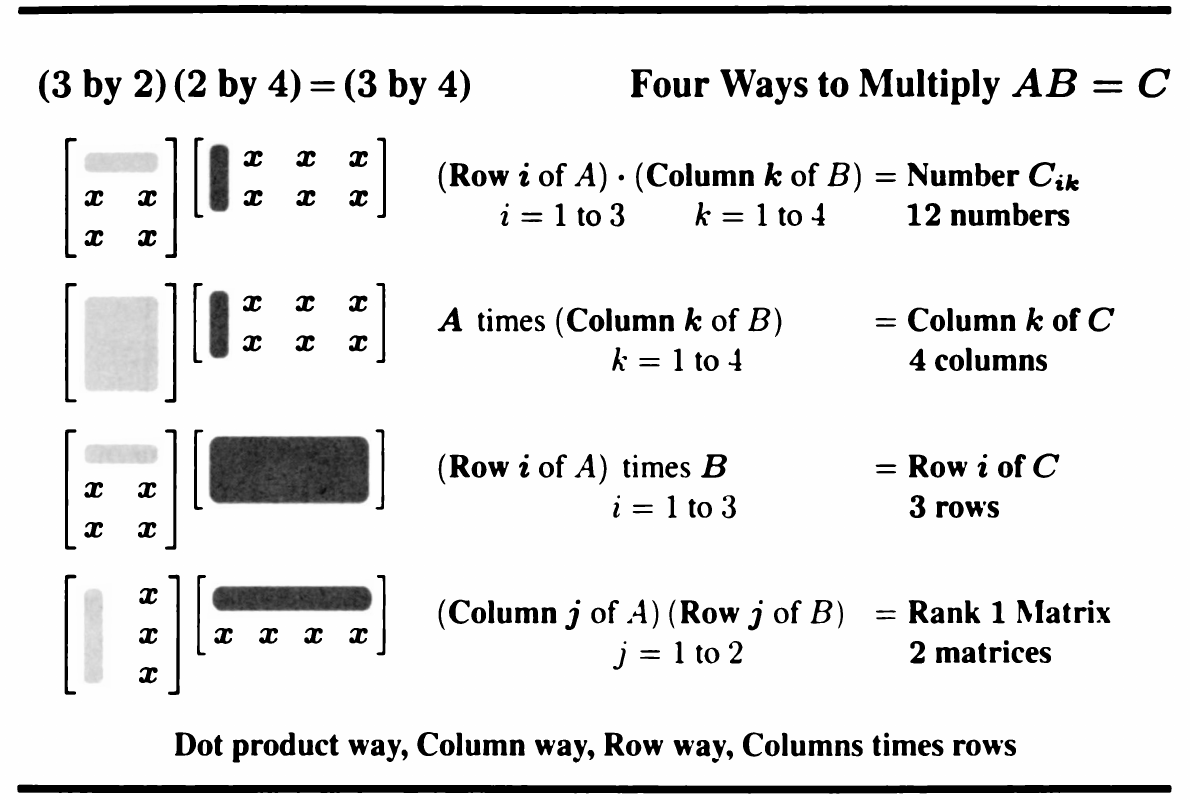
\includegraphics[width=10cm]{4}
\end{center}
(A nice way to intuit the the third method is to consider $(\bm{AB})^T=\bm B^T\bm A^T$; where the columns of $(\bm{AB})^T$ are the rows of $\bm{AB}$)
\newpage

\section{Solutions to $\bm{Ax}=\bm b$}
Given a $n$x$n$ matrix $\bm A$ and an $n$x1 column vector $b$, there are three outcomes for the vector $\bm x$ that solves $\bm{Ax}=\bm b$.\\
\vspace{1mm}\\
First there may be \textit{no vector} $\bm x$ that solves $\bm{Ax}=\bm b$, or there may be exactly \textit{one} solution, or there may be \textit{infinitely many}
solution vectors $\bm x$. Here are the possibilities:\\
\vspace{1mm}\\
1. \textbf{Exactly one solution} to $\bm{Ax}=\bm b$ means that $\bm A$ has independent columns (only one particular linear combination of the columns of $\bm A$
leads to $\bm b$. That combination is specified by $\bm x$). $\bm A$ is full rank and the only solution to $\bm{Ax}=\bm{0}$ is $\bm x=\bm0$. 
$\bm A$ \textit{has an inverse matrix} $\bm A^{-1}$ (given $\bm b$, we can work backward to get $\bm x$ since only one $\bm x$ leads to $\bm b$).\\
\vspace{1mm}\\
2. \textbf{No solution} to $\bm{Ax}=\bm b$ means that $\bm b$ is not in the column space of $\bm A$, so $\bm A$ is not full rank.\\
\vspace{1mm}\\
3. \textbf{Infinitely many solutions}. See that when the columns of $\bm A$ are not independent (not full rank), then there are infinitely many ways to
produce the zero vector $\bm b=\bm0$ (this is the meaning of dependent columns), and so there are infinitely many solutions to $\bm{AX}=\bm0$.\\
\vspace{1mm}\\ 
Also see that if $\bm A$ is not full rank it means that its column space is some subspace, where
solutions only exist for $\bm b$ within that subspace.\\
\vspace{1mm}\\
As such, if there so happens to be a solution to $\bm{Ax}=\bm b$ then we can add any solution to $\bm{AX}=\bm0$:
\begin{equation*}
\bm A(\bm x+\alpha\bm X)=\bm A\bm x+\alpha\bm A\bm X=\bm b+\bm0=\bm b
\end{equation*}
For some constant $\alpha$, which gives us $\bm b$ again---we have infinitely many solutions.
\newpage

\section{Elimination by elimination matrices}














\end{document}
